\documentclass[10pt,a4paper]{article}
\usepackage{fontspec}
\usepackage{amsmath,bm}
\usepackage{amsfonts}
\usepackage{amssymb}
\usepackage{graphicx}
\usepackage{subcaption}
\usepackage{hyperref}
\usepackage{cleveref}
\usepackage{lmodern}
\usepackage{placeins}
\usepackage{movie15}
\usepackage[left=1.00in, right=1.00in, top=1.00in, bottom=1.00in]{geometry}
\title{Assignment 1}
\author{Daniel Celis Garza}
\date{\today}
\begin{document}
	\maketitle
	\section{Part a}
	Because the magnetic field lines point in the standard $z-$direction (out of the page), the Larmor orbits of the positive particles go clockwise, while the negative particles girate anticlockwise. The Larmor radius, $r_{L} = \dfrac{m v_{\perp}}{q B}$ depends on the mass, therefore assuming a pure hydrogen plasma, the electrons would orbit with a radius $\sim 1840$ smaller than the protons. The inverse relationship between $r_{L}$ and the strength of the magnetic field $B$, means that the stronger the magnetic field, the smaller the Larmor radius. By combining these three pieces of information we may build an intuitive picture of what happens when the plasma is subject to a magnetic field which points in the standard $z-$direction and whose magnitude decreases as $x$ increases. In \cref{f:larmor} we can see a rough sketch of how the Larmor radius is smaller the closer the particle is to the left, producing a tear-drop shape, the effect is a a gradual shifting of the Larmor orbit's guiding centre. Over greater distances, the shape of the orbits would expand in a conical way as the particles move away from the higher field strength. \Cref{f:gradb} shows a smoothed representation of the $\nabla B$ drift.
	\begin{figure}[h!]
		\centering
		\begin{subfigure}[b]{0.6\textwidth}
			\centering
			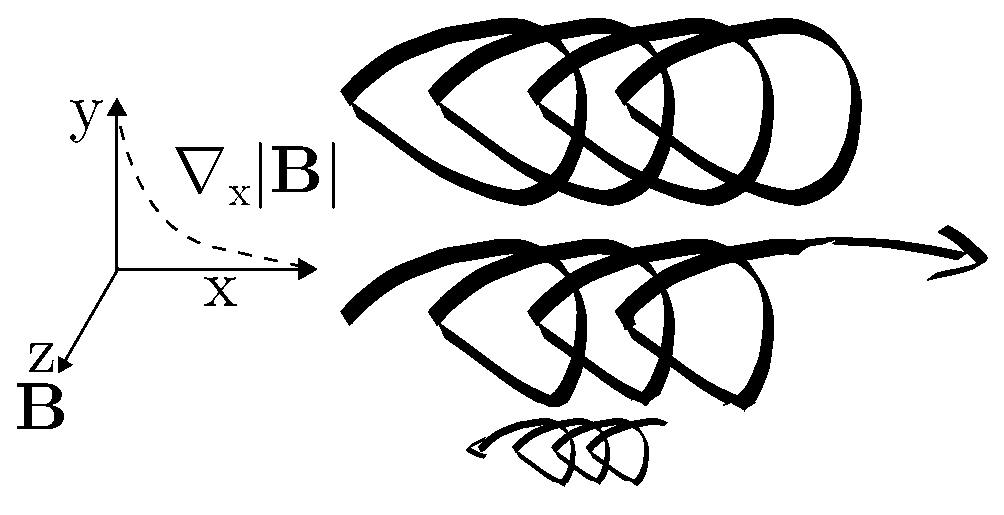
\includegraphics[width=\linewidth]{larmor.eps}
			\caption{Shape of the larmor orbits can be thought of as tear-drops, which result in a gradual drift in the direction of decreasing magnetic field strength.}
			\label{f:larmor}
		\end{subfigure}
		
		\begin{subfigure}[b]{0.7\textwidth}
			\centering
			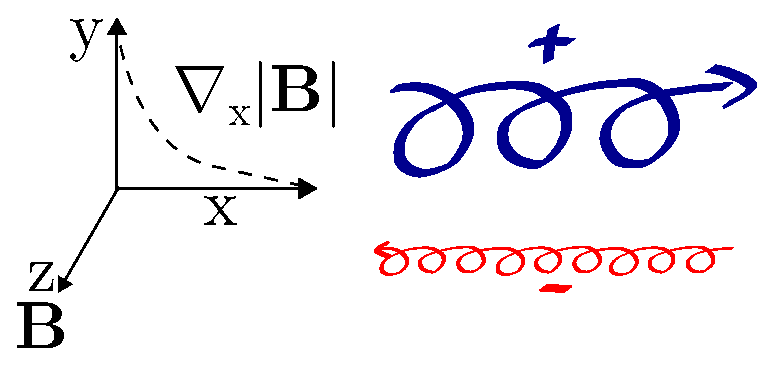
\includegraphics[width=\linewidth]{parta.eps}
			\caption{Diagram of $\nabla \bm{B}$ drift for positive and negative particles.}
			\label{f:gradb}
		\end{subfigure}
		\caption{$\bm{B}$ points in the $z-$direction (out of the page) and its magnitude decreases as $x$ increases (dashed line).}
		\label{f:gradbexp}
	\end{figure}
	
	\section{Part b}
	\subsection{I}
	Taking the definitions in \crefrange{e:vnabb}{e:vc} and evaluating with the purely toroidal field in \cref{e:b}, after going through the calculations in \crefrange{e:calcstart}{e:calcend}, substituting back into \crefrange{e:vnabb}{e:vc} and working through the algebra we obtain \crefrange{e:vnabbf}{e:vcf}. 
	
		\begin{align}
			\bm{V}_{\nabla B} &= \dfrac{r_{L} v_{\perp}}{2} \dfrac{B \times \nabla B}{B^{2}} \label{e:vnabb}
			\\
			\bm{V}_{c} &= \dfrac{m v_{\parallel}^{2}}{Z e B^{2}} \dfrac{R \times B}{R^{2}}
			\label{e:vc}
		\end{align}
		
		\begin{align}
			B &= \dfrac{C}{R} \bm{\nabla \phi} \Rightarrow B_{\phi} = \dfrac{C}{R}
			\label{e:b}
		\end{align}
		
		\begin{align}
			B_{\phi}^{2} &= \dfrac{C^{2}}{R^{2}} \label{e:calcstart} \\
			\nabla B_{\phi} &= \dfrac{\partial }{\partial R} \left(\dfrac{C}{R}\right) \bm{\nabla R} = - \dfrac{C}{R^{2}} \bm{\nabla R} \\
			B_{\phi} \times \nabla B_{\phi} &= 
				\begin{vmatrix}
					\bm{\nabla R} & \bm{\nabla \phi} & \bm{\nabla z} \\
					0 & \dfrac{C}{R} & 0 \\
					-\dfrac{C}{R^{2}} & 0 & 0
				\end{vmatrix} = \dfrac{C^{2}}{R^{3}} \bm{\nabla z} \\
		imagefile	R \times B_{\phi} &= 
				\begin{vmatrix}
					\bm{\nabla R} & \bm{\nabla \phi} & \bm{\nabla z} \\
					R & 0 & 0 \\
					0 & \dfrac{C}{R} & 0
				\end{vmatrix}  = C \bm{\nabla z}
				\label{e:calcend}
		\end{align}
		
		\begin{align}
			r_{L} &= \dfrac{m v_{\perp}}{Z e B} \\
			\bm{V}_{\nabla B} &= \dfrac{r_{L} v_{\perp}}{2} \dfrac{1}{R} \bm{\nabla z} =  \dfrac{m v_{\perp}^{2}}{2 Z e C} \bm{\nabla z} \label{e:vnabbf} \\
			\bm{V}_{c} &= \dfrac{m v_{\parallel}^{2}}{Z e C} \bm{\nabla z} \label{e:vcf}
		\end{align}
		
		Under these conditions, the drift velocities depend on charge in the $\bm{\nabla z}$ direction, therefore ions and electrons will drift in opposite directions! Positive ions will drift in the positive direction, while electrons will drift in the negative one. This charge separation will generate an electric field in the plasma as observed in the sketch in \cref{f:efield}.
		\begin{figure}[h!]
			\centering
			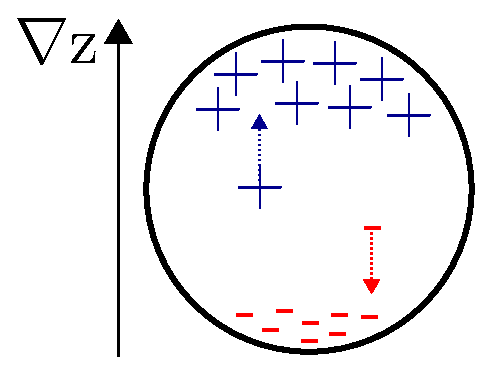
\includegraphics[width=0.4\textwidth]{drift.eps}
			\caption{Under a purely toroidal magnetic field, the cross B drift causes a charge separation within the plasma.}
			\label{f:efield}
		\end{figure}
		\subsection{II}
		In order to counteract this drift---and thus improve the plasma confinement---we induce a polloidal field by passing a current through the plasma as shown in \cref{f:totalb}. The resulting magnetic field lines are a linear combination of the coordinates (resulting in m\"{o}bius-like field lines) and serve to rotate the $\bm{\nabla z}$ direction such that the average drift of the charged particlclose to $0$ andes is as small as possible, thus keeping the electric field as close to $0$ as we can.
		\begin{figure}
			\centering
			\begin{subfigure}[b]{0.45\textwidth}
				\centering
				\includegraphics[width=0.5\textwidth]{toroidal_coord.png}
				\caption{Toroidal coordinate shown in blue and polloidal coordinate shown in red.}
			\end{subfigure}
			~
			\begin{subfigure}[b]{0.45\textwidth}
				\centering
				\includegraphics[width=0.5\textwidth]{tokamak_field.png}
				\caption{Adding a polloidal magnetic field results in the total magnetic field.}
			\end{subfigure}
			\caption{Total magnetic field in a tokamak.}
			\label{f:totalb}
		\end{figure}
		
	\section{Part c}
	Starting from the Maxwellian distribution in \cref{e:maxw}, assuming a small aspect ratio $\epsilon$, and using \crefrange{e:vlim1}{e:vlim2} to find the integration limits necessary for confinement ($v_{\parallel} \leq 0$) in terms of $v_{\perp}$.
	\begin{align}
		f(v) = \dfrac{1}{(2 \pi)^{3/2}} \dfrac{1}{v_{th}^{3}} \exp \left(- \dfrac{v^{2}}{2 v_{th}^{2}}\right)
		\label{e:maxw}
	\end{align}
	\begin{subequations}
		\begin{align}
			v_{\parallel}^{2} &= v^{2} \left(1 - \dfrac{v_{\perp}^{2}}{v^{2}} \dfrac{1 - \epsilon \cos(\theta)}{1-\epsilon}\right) \label{e:vlim1}\\
			v_{\parallel}^{2}(\theta = 0) &= v^{2} \left(1 - \dfrac{v_{\perp}^{2}}{v^{2}} \dfrac{1+\epsilon }{1-\epsilon}\right) \\
			\textrm{if } \dfrac{1+\epsilon }{1-\epsilon} &\leq \dfrac{v^{2}}{v_{\perp}^{2}}  \textrm{ then } v_{\parallel} \leq 0 \\
			v^{2} &= v_{\perp}^{2} + v_{\parallel}^{2} \\
			\dfrac{1 - \epsilon }{1-\epsilon} + \dfrac{2 \epsilon}{1-\epsilon} &\leq \dfrac{v_{\perp}^{2}}{v_{\perp}^{2}} + \dfrac{v_{\parallel}^{2}}{v_{\perp}^{2}} \\
			- v_{\perp} \sqrt{\dfrac{2\epsilon}{1-\epsilon}} \leq &v_{\parallel} \leq \pm v_{\perp} \sqrt{\dfrac{2\epsilon}{1-\epsilon}}
			\label{e:vlim2}
		\end{align}
	\end{subequations}
	We integrate the volume in cylindrical coordinates (torus is a cylinder connected on its two faces), setting the integration limits on the velocities to be $0 \rightarrow \infty$ for $v_{\perp}$ as we want all perpendicular velocities and using the limits derived in \cref{e:vlim2} for $v_{\parallel}$ as we want to know the trapped fraction of particles.
	\begin{subequations}
		\begin{align}
			F_{t}(v) &= \dfrac{1}{(2 \pi)^{3/2}} \dfrac{1}{v_{th}^{3}} \int\limits_{0}^{2\pi} \mathrm{d}\phi \int\limits_{0}^{\infty} v_{\perp} \exp\left(- \dfrac{v_{\perp}^{2}}{2 v_{th}^{2}}\right) \mathrm{d}v_{\perp} \int\limits_{-v_{\perp} \sqrt{\dfrac{2\epsilon}{1-\epsilon}}}^{v_{\perp} \sqrt{\dfrac{2\epsilon}{1-\epsilon}}} \exp\left(- \dfrac{v_{\parallel}^{2}}{2 v_{th}^{2}}\right) \mathrm{d}v_{\parallel} \\
			F_{t}(v) &= \dfrac{4}{\sqrt{\pi}} \int\limits_{0}^{\infty} \dfrac{v_{\perp}}{\sqrt{2} v_{th}} \exp\left(- \dfrac{v_{\perp}^{2}}{2 v_{th}^{2}}\right) \mathrm{d}\left(\dfrac{v_{\perp}}{\sqrt{2} v_{th}}\right) \int\limits_{0}^{\dfrac{v_{\perp}}{\sqrt{2} v_{th}} \sqrt{\dfrac{2\epsilon}{1-\epsilon}}} \exp\left(- \dfrac{v_{\parallel}^{2}}{2 v_{th}^{2}}\right) \mathrm{d}\left(\dfrac{v_{\parallel}}{\sqrt{2} v_{th}}\right) \\
			s &= \dfrac{v_{\parallel}}{\sqrt{2} v_{th}} \qquad t = \dfrac{v_{\perp}}{\sqrt{2} v_{th}} \\
			F_{t}(v) &= \dfrac{4}{\sqrt{\pi}} \int\limits_{0}^{\infty} t e^{-t^{2}} \mathrm{d}t \int\limits_{0}^{t \sqrt{\dfrac{2\epsilon}{1-\epsilon}}} e^{-s^{2}} \mathrm{d}s \\
			F_{t} &= \dfrac{4}{\sqrt{\pi}} \int\limits_{0}^{\infty} t e^{-t^{2}} \mathrm{d}t \dfrac{\sqrt{\pi}}{2} \textrm{erf}\left(t \sqrt{\dfrac{2\epsilon}{1-\epsilon}}\right) \\
			&\textrm{Taylor expand } \dfrac{\sqrt{\pi}}{2}\textrm{erf}\left(t \sqrt{\dfrac{2\epsilon}{1-\epsilon}}\right) \textrm{ to $O(n)$ (one term) around } t = 0 \nonumber\\
			F_{t} &\approx \dfrac{4}{\sqrt{\pi}} \sqrt{\dfrac{2\epsilon}{1-\epsilon}} \int\limits_{0}^{\infty} t^{2} e^{-t^{2}} \mathrm{d}t = \sqrt{\dfrac{2\epsilon}{1-\epsilon}} \\
			&\textrm{Taylor expand around $\epsilon = 0$} \nonumber\\
			F_{t} &\approx 2\epsilon
		\end{align}
	\end{subequations}
	
	Tokamak magnetic fields are non-uniform curved fields, as a result the poloidal field prevents the $\bm{E} \times \bm{B}$ drift but not the total drift. As a result, particles still move away from the flux surfaces, causing some particles to be trapped in so called ``banana orbits'' \cref{f:banana}. Within these orbits, particles collide more often than they would in a bulk plasma. It is useful to define the conditionality of a banana orbit as the ratio between the period of the banana orbit to the average time between collisions which result in detrapping,
	\begin{align}
		\nu_{*} &= \dfrac{t_{b}}{\tau_{eff}} = \nu_{eff} t_{b}\\
		t_{b} &\sim \dfrac{R q}{\sqrt{\epsilon} v_{th}}\\
		\nu_{*} &= \dfrac{\nu}{\epsilon^{3/2}} \dfrac{Rq}{v_{th}}
		v_{th} &\sim \sqrt{\dfrac{T_j}{m_j}}~.
	\end{align}
	Ion-ion collisions $\nu_{*} \propto \dfrac{n}{T^2}$, which means that in large, hot tokamaks trapped particle effects become important. Fortunately, having trapped particles in defined orbits improves containment time, and allows currents to be driven inside the plasma more effectively. Furthermore, collisions between particles in adjacent banana orbits improve the in-plasma current even further in a self-sustaining fashion. This is the bootstrap current and it depends on the density of the plasma in adjacent banana orbits and is described by $J_{b} = \epsilon^{1/2} \dfrac{T}{B_{0}} \dfrac{\mathrm{d} n}{\mathrm{d} r}$, and is the result of momentum transfer and friction between particles in adjacent banana orbits. The motivation behind making bigger and bigger tokamaks is a consequence of the search for a self-sustaining current and longer confinement times.
	\begin{figure}
		\centering
		\includegraphics[width=0.5\textwidth]{banana.jpg}
		\caption{Example of a banana orbit.}
		\label{f:banana}
	\end{figure}
	
\end{document}